% Fourier Analysis Introduction
In the beginning of the 1800s, Joseph Fourier was working on a physics problem called the heat equation, a certain partial differential equation. He had the idea of expressing the original function as a sum of sine and cosine functions as these would integrate and differentiate easily, making the differential equation easier to solve. He eventually developed and introduced the idea of Fourier series, a way of expressing a function as a sum of trigonometric functions \cite{Bounchaleun2019}.

% Fourier Series
\subsection{Fourier Series} 
If a function has a period of $2\pi$, the Fourier series takes the form $$f(t) = \frac{a_0}{2} + \sum_{n=1}^{\infty}a_ncos(nt)+\sum_{n=1}^{\infty}b_nsin(nt)$$ and states that a function can be represented by an infinite number of sine and cosine waves with different magnitudes and coefficients, plus some constant term. To compute the coefficients, the following formulae are used
$$a_0 = \frac{1}{\pi}\int_0^{2\pi} f(t)dt$$
$$a_m = \frac{1}{\pi}\int_0^{2\pi} f(t) sin(mt)dt$$
$$n_m = \frac{1}{\pi}\int_0^{2\pi} f(t) cos(mt)$$

which may be derived using the properties of a few integrals of trigonometric functions.

A sawtooth wave is perhaps the easiest to demonstrate the computations on, as it is simply $f(t) = t$ over the interval. The constant term is $\frac{1}{\pi}\int_0^{2\pi} t dt = 2\pi$. The first $a_m$ term is the result of $\frac{1}{\pi}\int_0^{2pi} t sin(1t)dt = -2$, which may be done using integration by parts. The subsequent $a_m$ sine terms repeat the exact same step with different values of $m$. For this function, all cosine terms are 0, since $f(t)=tcos(t)$ is an odd function. The fourier series for this kind of sawtooth wave is thus
$$\pi + -2sin(t) -1sin(2t)-\frac{2}{3}sin(3t) - \frac{1}{2}sin(4t) ...$$

This approach, in a general sense, can be used to find the coefficients for other functions.
 
% \cite{SimonXu2015}

% Fourier Transform
\subsection{Fourier Transform} 
The Fourier Transform is an operation that takes a function in time domain (a signal as a function of time, like a sound) and outputs a function in frequency domain, a kind of description for which kinds of sinusoids make up the original signal. Figure \ref{fig:transform} shows a signal and its corresponding frequency-domain representation. The right diagram is a frequency-magnitude plot where the x-coordinate represents frequency and the y-coordinate represents the magnitude of the complex output of the transform. The peaks in the frequency domain shows that the signal is composed of the sinusoids $10sin(2\pi * 50t)$, $2sin(2\pi * 150t)$, $5sin(2\pi * 300t)$ and a significant amount of noise. In other words, the signal contains frequency components of 50Hz, 150Hz and 300Hz. 

\begin{figure}[ht]
    \centering
    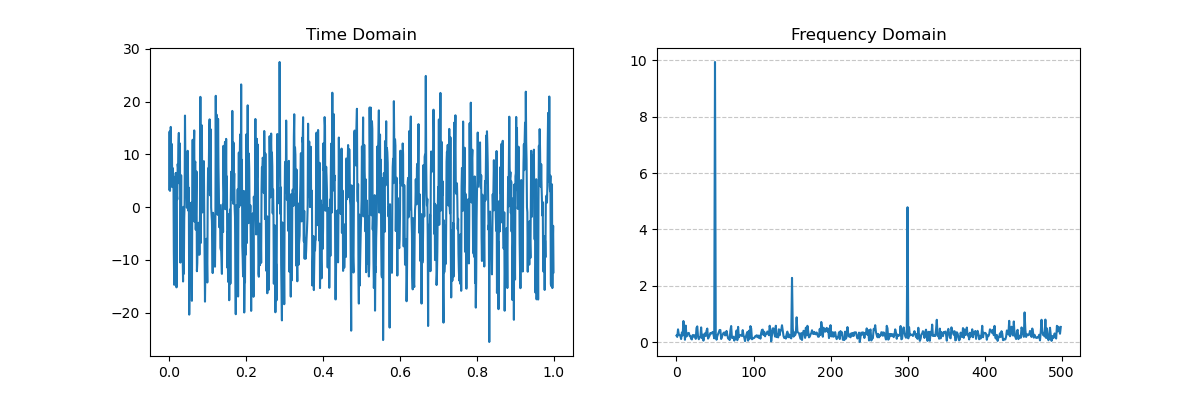
\includegraphics[width=\textwidth]{./images/transform.png}
    \caption{Some signal in the time-domain (displayed on the left) with added noise. Computing the transform with a discrete version of the Fourier transform reveals the main frequencies that make up the original signal in the time-domain (displayed on the right)\label{fig:transform}}
\end{figure}

Even though the the Fourier transform is an incredibly powerful function, its formula is compact. 
$$\hat{f}(x) = \int_{-\infty}^{\infty} f(t)e^{-i2\pi x t} dt$$
It's worth noting at this point that \textit{transform} refers both to the act of transforming the function between domains but sometimes also the output values are called the transform. The time-domain to frequency-domain transform is sometimes called the forward transform to emphasize the direction of the transform as the inverse (frequency-domain to time-domain) is also called a transform.

% High level description of the Fourier transform.
\subsubsection{The big idea}
For the sake of simplicity, let's assume an interval of $[0, 2\pi]$. The following equations help explain what the Fourier transform does.
\[ \int_0^{2\pi} sin(mx)sin(nx)dx = \int_0^{2\pi} cos(mx)cos(nx)dx= 
\begin{cases} % Some issues with cases
    0 & m\neq n \\
    \pi & m=n
\end{cases} 
\]
\noindent and
$$\int_0^{2\pi} sin(mx)cos(nx)dx = 0$$

If $n = m $, $sin(nx), n\in\mathbb{Z}$ will interfere with $sin(mx), m\in\mathbb{Z}$, and integrating over the interval yields $\pi$. If $n \neq m$, integrating over the interval gives 0. When the signals are independent, when the definite integral equals 0, they are said to be orthogonal. When they are non-orthogonal, they correlate. 

Intuitively, the Fourier transform is a function that checks correlation between another signal and all sinusoids. For example, transforming the signal $sin(440t)$, yields a 0 for every sinusoid, except $sin(440t)$, which means that $sin(440t)$ is part of the original signal.

\begin{figure}[ht]
    \centering
    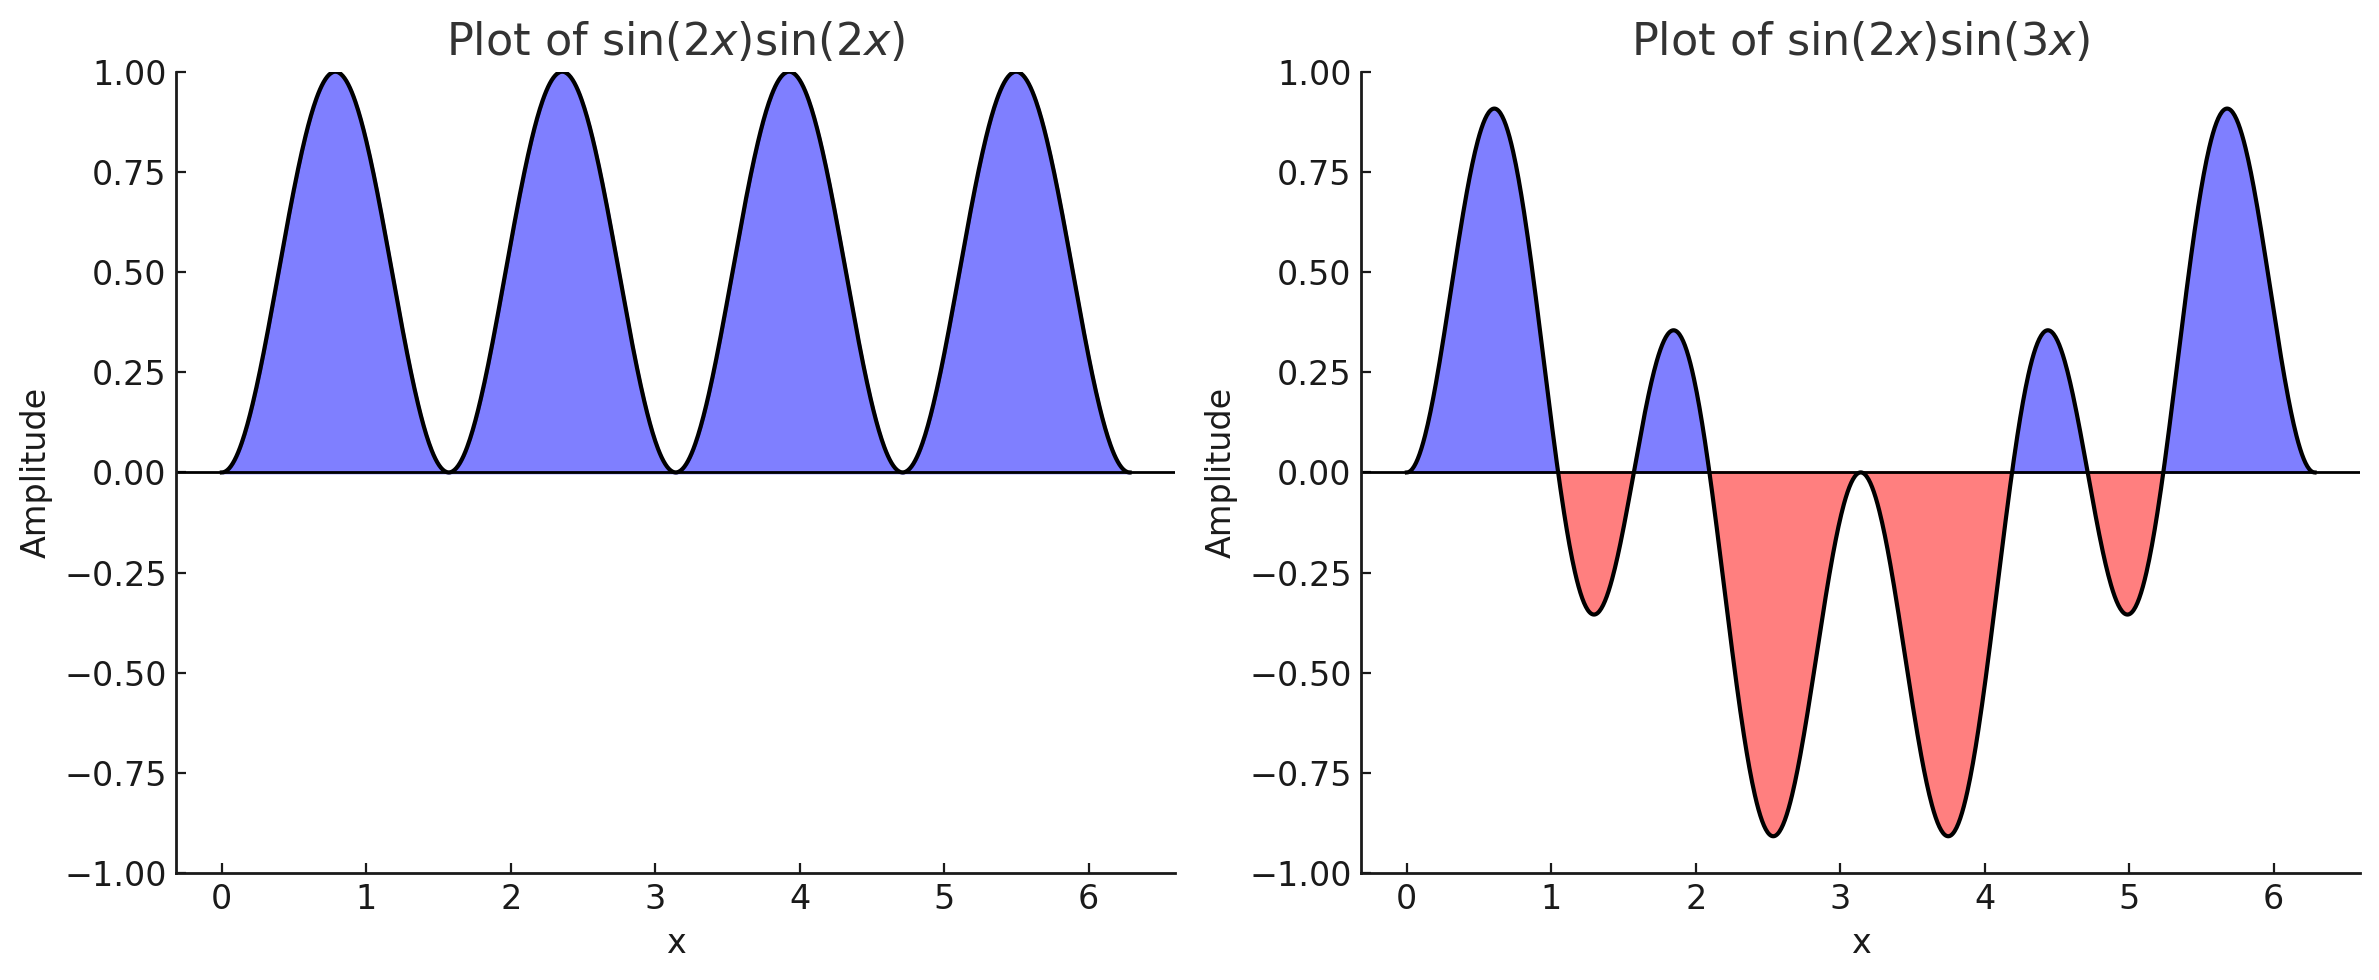
\includegraphics[width=\textwidth]{./images/transformIdea.png}
    \caption{The graphs of $sin(2x)sin(2x)$ and $sin(2x)sin(3x)$ on the $0$ to $2\pi$ interval. Matching $n$ and $m$ results in $sin^2(2x)$ which is always positive, resulting in a positive area whereas a mismatch causes equal positive and negative area, canceling out to 0.\label{fig:transformIdea}}
\end{figure}

% DFT
\subsection{Discrete fourier transform} 
The Discrete Fourier transform (abbreviated as DFT), as the name implies, is the Fourier transform for discrete signals. Instead of integrating over the entire function domain, we sum the samples from the signal starting from the start of the signal at $t=0$ to some $t=N$. The DFT for a signal $x$ with $N$ points is 
$$X_k = \sum_{n=0}^{N-1} x_ne^{-\frac{i2\pi kn}{N}}$$

% Matrix
\subsubsection{Matrix representation for the DFT computations} 
The DFT can be represented and computed by a matrix-vector multiplication. 
$$
% DFT coefficients
\begin{bmatrix}
    X(0) \\
    X(1) \\
    X(2) \\
    X(3) \\
    \vdots\\
    X(n) \\
\end{bmatrix}
=
% DFT matrix
\begin{bmatrix}
    1 & 1 & 1 & 1 & \cdots & 1\\
    1 & \omega & \omega ^2 & \omega ^3 & \cdots & \omega ^n\\
    1 & \omega ^2 & \omega ^4 & \omega ^6 & \cdots & \omega ^{2n}\\
    1 & \omega ^3 & \omega ^6 & \omega ^9 & \cdots & \omega ^{2n}\\
    \vdots & \vdots & \vdots & \vdots & \ddots & \vdots \\
    1 & \omega ^{n} & \omega ^{2n} & \omega ^{3n} & \cdots & \omega ^{{n^2}}\\
\end{bmatrix}
% Discrete signal
\begin{bmatrix}
    x(0) \\
    x(1) \\
    x(2) \\
    x(3) \\
    \vdots\\
    x(n) \\
\end{bmatrix}
$$
where $n = N-1$ as the computation are zero-indexed and $\omega$ is the principle N-th root of unity $e^{2\pi i/N} $. 

% \todo{but why a matrix when the summation formula is both practical and more compact..? Also, FFT? What's the damn point?}

% Inverse transform
\subsection{Inverse Transforms}
The time-domain signal can be used, transmitted, received, but is hard to work with. The frequency domain on the other hand is easy to work in, but makes little to no sense in many use cases. A C-major chord in the frequency domain can not be played, for example. The forward Fourier transform allows the transformation from time to frequency domain, but once any modification (like high frequency filtering) is applied, the signal needs to be transformed back to the time domain in order to be useful. The operation that does this is appropriately called the inverse Fourier transform, IFT for short or IDFT, for the discrete variant.

The inverse Fourier transform is very similar to the forward Fourier transform:
$$ f(t) = \frac{1}{\pi}\int_{-\infty}^{\infty} \hat{f}(\zeta)e^{i2\pi\zeta t} d\zeta$$
and the discrete inverse transform is 
$$ x_n = \frac{1}{N}\sum_{k=0}^{N-1} X(k)e^{\frac{i2\pi kn}{N}}$$

the only difference is a normalization factor and negation of the exponent.

% Computing
\subsection{Computations}
For pretty much any practical usage of the DFT, so many samples will be used that it's not feasible to compute by hand. The DFT computations thus need to be converted to an algorithm or similar programmatic construct a computer can understand and run.

\subsubsection{Example DFT using the formula}
The formula is technically easy to use both in manual computations and when writing software for it. Given a discrete input signal 

$$x = [-0.01298834,  0.62287525,  0.64266088,  0.39309558,  0.55407458, \cdots]$$

which has a 100 elements, the DFT values can be computed with the formula $$X_k = \sum_{n=0}^{N-1} x_ne^{-\frac{i2\pi kn}{N}}$$. Starting with $k=0$ $X_0 \approx -0.3215+0i$, a number with both the real and imaginary components close to 0, which indicates very little impact on the original signal. At $k=5$ however, $X_k \approx 0.07725-24.5836i$ with a relatively large imaginary component. Repeating the same summation up to $k=100-1 = 99$ the other values of $X_k$ with relatively large imaginary components are at $k=12$ and $k=25$. 

To obtain the frequency-magnitude plot, which simply will be referred to as the \textit{spectrum} from here on, the magnitudes for each complex valued $X_k$ are needed. The magnitude represents the length of the equivalent vector of the DFT values, and since the vector forms a right triangle, the length of the vector (or hypotenuse of the triangle) can be computed using the Pythagorean theorem $a^2 + b^2 = c^2$. 

% Nyquist thing here

\subsubsection{Computing DFT with a programming language}
With the built-in complex data types and extensive mathematical and scientific computing libraries, implementing the DFT in Python is trivial. Leveraging Python's cmath library, the computations can be copied directly and 2 for-loops handles the summation and $X_k$ indexing as shown below.

\lstinputlisting[style=python]{../snippets/dft-A.py}

For a more primitive language like C, without complex exponentiation, the computations are still fairly straightforward to do due to Euler's formula that expands $e^{ix} = cos(x) + isin(x)$. The components can be separated into two separate data structures and so the imaginary unit can be dropped. A possible C implementation (without using a struct for complex numbers) is shown below. 

\lstinputlisting[style=c]{../snippets/dft-A.c}

These examples are purely illustrative, there is no reason to use the DFT in practice because there are algorithms that do the same transformation with significantly less computation, and the efficiency improvement grows with the input size.

\subsubsection{Computing the inverse}

Writing the inverse discrete Fourier transform in Python is as trivial as the DFT due to the cmath library. Like the formula, the algorithm is mostly the same, but with normalization and a negated exponent.

\lstinputlisting[style=python]{../snippets/dft-C.py}

The inverse may be used after processing the frequency domain. For demonstration purposes, the signal has been filtered by removing any component that has a magnitude under a certain threshold. Figure \ref{fig:DFT-IDFT} shows both the original signal and filtered signal in both time and frequency domain. One can observe less noise in the blue time-domain signal.

\begin{figure}[ht]
    \centering
    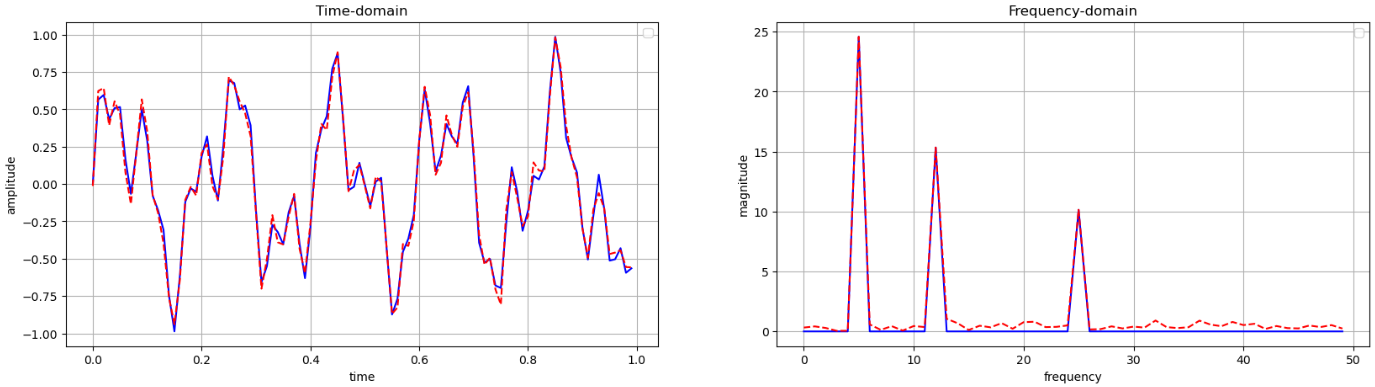
\includegraphics[width=\textwidth]{./images/filtered_signal.png}
    \caption{The time-domain and frequency-domain representations of the signal (red dashed line) and the filtered signal (blue solid line)\label{fig:DFT-IDFT}}
\end{figure}

% FFT
\subsection{Fast fourier transform}
The DFT takes $n^2$ operations to perform as there are $n$ outputs $X_k$ and $n$ amount of numbers to be summed. A fast fourier transform (abbreviated as FFT) is any method that speeds up the computation of the DFT. This means that even if there is one Fourier transform and basically one DFT, there are multiple FFT algorithms. Arguably, very few users of the FFT cares about the implementation, they just expect the functionality of the DFT, but faster. 

\subsubsection{Time complexity}
Time complexity refers to the asymptotic performance of an algorithm. Even though it often correlates with performance, it is ultimately theoretical and only considers the highest-order term, because it is the greatest contributor when the input size grows towards infinity. For example, consider an algorithm for multiplying 2 numbers. One such algorithm, commonly taught in elementary school, multiplies every digit of one operand with every digit of the other. The result of each multiplication is added to the previous, accounting for carrying, to form a single number. This process results in an array of numbers, each of which is a multiple of a power of 10. The final step of the algorithm is to sum these numbers. The first step takes $N^2$ operations, where $N$ is the length of the operands (assuming they are the same length), and the second step takes $N$ operations. This algorithm thus takes $N^2+N$ steps but as N grows larger and larger, the $N^2$ term will contribute the most, so we say that the algorithm has a complexity of $O(N^2)$, which is referred to as \textit{Big-O}. For example, multiplying two 1000-digit long integers, the multiplication will take a million operations and the summation will take 1000. Increasing the input size with 1 digit adds only 1 more addition, but it adds 1001 more multiplication steps.

Perhaps the most popular algorithms, the Cooley-Tukey FFT, has an algorithmic complexity of $O(n \log n)$, a significant speed up over $O(n^2)$ \cite{Randhawa2018} \cite{HeidemanEtAl1984}. Once in Big-O, the base of the logarithm does not matter, what matters is that it is logarithmic. An improvement from $O(n^2)$ to $O(n \log n)$ means that even with a mere 1000 samples, the speed up, purely in terms of time complexity, is approximately 100x. In a paper by James Cooley, he exemplified a computation with the Fourier transform on a dataset of 512,000 data points which he claims would see an approximately 12,800x speedup with the FFT \cite{Cooley1987}. 512,000 data points would take on the order of 262 billion operations to complete with an $O(n^2)$ algorithm, which with a modern personal computer can take minutes to complete. An $O(n \log n)$ algorithm takes a relatively measly 9.7 million operations and runs in milliseconds. This is akin to measuring the execution time of Quick sort to Bubble sort for an array of size 512,000 which indeed sees a speedup of this magnitude.

This speedup in execution time and theoretical time complexity improvement demonstrates the power of the FFT. Why this improvement is so important will, hopefully, be evident later.. Essentially, the FFT is considered by some to be one of the most important algorithm of all time due to being able to perform very important heavy computations instantaneously. 

% \subsubsection{Brief history of the FFT} \todo{this whole section is bad, I'll either fix it or remove it later}
% The history of the FFT is long and cloudy with multiple scientists working on a similar problem between 1800-2000. Cooley and Tukey introduced their algorithm in 1965 and at the time it was regarded as a completely new and revolutionizing algorithm. Based on the papers [A] and [B], the FFT and similar numerical methods were developed in two chains. One of them was started with Euler and Lagrange which Gauss based his work on. Runge's work is based on ????????? Gauss and was the basis for a lot of other development. The other chain, which seemingly does not link to Gauss is where Cooley-Tukey exists. They tributed I.J. Good in their paper even though their algorithm was pretty different from the Good one, which is now commonly called the Prime Factor Algorithm and sometimes Good-Thomas. 

% % Yates used? FFT for a convolution

% It was later discovered that Cooley-Tukey works almost exactly as the algorithm Gauss had proposed almost a century earlier. This is probably why Cooley talks about the "re-discovery" in one of his paper. Since the algorithm was only rediscoverd by Cooley and Tukey, some would like to give Gauss more credit for the FFT and some authors have used terms such as "Discrete Gauss Transform (DGT)" and "Gauss-Fourier Transform (GFT)". To make the history of the FFT even muddier, Clairaut published a cosine-only "DFT" 50 years before Fourier even came forth with the Fourier series. Lagrange came up a sine-only DFT-like formula around 40 years before Fourier series.

% At first, the Cooley-Tukey algorithm was regarded as an entirely new thing.   
% The modern FFT (what's that?) is based on the work of Gauss, almost which was developed almost a century before Cooley-Tukey. Gauss and CT use the same algorithm but the equivalence is not obvious due to Gauss' obscure and outdated notation.

% Some would like to credit Gauss with the FFT even though it would be impractical. Some have and there have been uses of the terms "Discrete Gauss transform (DGT)" and " Gauss-Fourier transform (GFT)".

% In the 1800s, an FFT which was NOT based on Gauss was widely used

% Clairaut published a cosine-only "DFT" in 1754, 50 years BEFORE Fourier's Fourier series??? Lagrange came with a sine-only DFT-like formula in 1762


% CT > Good > Thomas, Yates
% Rudnick > Danielson-Lanczos > Runge 
% Gauss > Lagrange, Euler
% Smith > Darwin > Thompson > Runge
% Smith > Everett > Darwin & Smith > Kelvin > Everett > Darwin
% What is the link between Thomas, Yates and the "rest"?
% What's the link between Gauss and Runge
% Where does Carlini fit into the picture?

\subsubsection{FFT Algorithm}
As previously mentioned, FFT is simply put any algorithm that computes the DFT \textit{fast}. One of the easier to understand while still demonstrating the workings of the algorithm is the Radix-2 FFT. The Radix-2 FFT is easy to understand because it assumes the input size is a power of 2, meaning it's easy to recursively split into two. On a high level, the Radix-2 algorithm starts with splitting the input array into odds and evens. It then calls itself for the odds and evens, recursively splitting the array until it performs FFTs on arrays of length 1. On the way back up, it performs the DFT on smaller units of the original signal, utilizing the symmetry of roots of unity and values that it has already computed to perform multiple operations at once. 

The following mathematical derivation of the Radix-2 FFT is adapted from \cite{Rozman2019}. It starts with splitting the DFT into two sums, one for the even indices and one for the odd 
$$X_k = \sum^{N/2-1}_{n=0} x_{2n}T^{2n}+ \sum^{N/2-1}_{n=0} x_{2n+1}T^{2n+1}$$
where $T_k$ is the so called twiddle factor $e^{-\frac{2\pi ik}{N}}$. A common twiddle factor is factored out of the odd sum and the even and odd sums are denoted as $E_k$ and $O_k$ respectively. 

$$X_k = E_k + T_kO_k$$

These functions $E_k$ and $O_k$ are periodic with a period $N/2$ which can be shown by showing that $$e^{\frac{-2\pi in(k+N/2)}{N/2}} = e^{\frac{-2\pi in(k)}{N/2}}$$
which means that 
$$E_k = E_{k+\frac{N}{2}}, O_k = O_{k+\frac{N}{2}}$$
and since this holds true for $E_k$ and $O_k$, the following is also true

\[
X_k = \left\{\begin{array}{lr}
    E_k + T_kO_k, & \text{for } 0 \leq k < N/2\\
    E_{k-N/2} + T_kO_{k-N/2}, & \text{for } N/2\leq k< N\\
    \end{array}\right\}
\]

This implies that the DFT can be computed in two layers (for lack of a better term), the lower $N/2$ terms and the upper $N/2$ terms.
When computing the upper $N/2$ terms, i.e. when $N/2 \leq k < N$, $X_k = E_{k-N/2} + T_k^{N/2}O_{k-N/2}$, which are the same O and E as the lower $N/2$ terms, just with an offset of N/2. The twiddle factor is raised to the power of N/2 because it too is in terms of $k$. We can thus split $X_k$ into 
% \todo{This section could be reworked}

$$X_k = E_k + T_kO_k$$  
$$X_{k+N/2} = E_k + T_k^{N/2}O_k$$
which are the equations for the lower and upper $N/2$ terms. Finally the twiddle factor is rewritten using the following property of complex exponentials

$$e^{\frac{-2\pi i(k+N/2)}{N}} = -e^{\frac{-2\pi ik}{N}}$$
which gives

$$X_k = E_k + T_kO_k$$  
$$X_{k+N/2} = E_k - T_kO_k$$

Recall that

$$E_k = \sum^{N/2-1}_{n=0} x_{2n}T_k^{2n}$$
$$O_k = \sum^{N/2-1}_{n=0} x_{2n+1}T_k^{2n}$$
and that the DFT is
$$X_k = \sum^{N}_{n=0} x_nT^{n}$$

This means that when the element indeces are adjusted, $E_k$ and $O_k$ are both DFTs essentially. To transform this purely mathematical notation into something that looks more like a complete algorithm, the core computations are implemented with a loop

\begin{lstlisting}
do k = 0, N/2-1
    T = exp(-2*i * PI * k / N) 
    X(k+1) = E(k+1) + T * O(k+1)
    X(k+1 + N/2) = E(k+1) - T * O(k+1)
end do
\end{lstlisting}

In Fortran, arrays are indexed starting from 1, this means that every array access needs an offset of 1. Before these computations, the evens and odds must be computed.

\begin{lstlisting}
E = r2fft(input(1:N:2))
O = r2fft(input(2:N:2))
\end{lstlisting}

Any recursive algorithm also needs a base case to prevent the algorithm from looping indefinitely. In the case of the FFT, this is when the input array has a single value.

\begin{lstlisting}    
if (N == 1) then
    X = input
    return
end if
\end{lstlisting}

Putting everything together and adding variable declarations and initialization as well as the function declaration, a naive Radix-2 FFT could look like the following

\lstinputlisting[style=fortran, label={code:fortran-fft}]{../snippets/fft-A.f90}

This implementation assumes the input is a power of 2 but this is not handled anywhere. The program still runs, but to no surprise gives an erroneous answer. The algorithm can be visualized with a block diagram as shown in Figure \ref{fig:FFT-Alg}.

\begin{figure}[ht]
    \centering
    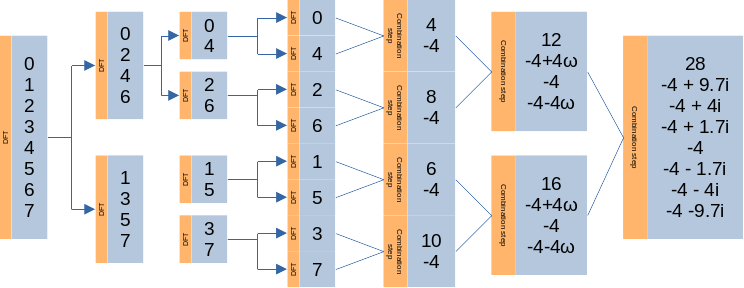
\includegraphics[width=\textwidth]{./images/fft.png}
    \caption{Diagram of a 4-point FFT. The process starts with splitting down the input vector to the recursive base case $N=1$. After that the values are combined using the core computations of the FFT.\label{fig:FFT-Alg}}
\end{figure}

\subsubsection{Time Complexity of Radix-2 FFT}
The FFT is ubiquitous, and the algorithm has been explored in depth. Literature explaining and deriving the algorithm exists and following it to implement the algorithm in code is almost trivial. It is easy to overlook the ingenuity of the algorithm and be fooled by the simplicity of it when seeing it written down. Where the $O(n\log n)$ complexity comes from might not be entirely clear even when seeing the algorithm written out in code because even, though the divide-and-conquer method splits into two, multiple computations are done within each function call. 

When taking a 4-point FFT, as shown in Figure \ref{fig:FFT-Alg}, the last combination step forming definitely needs four computations. One can also observe that each of the 2-point FFTs (which is a subproblem of the 4-Point FFT) takes 2 computations. All in all, it takes eight computations to compute the 4-point FFT. The total amount of computations for an 8-point FFT similarly is 8 plus 2 * number of computations of the 4-point FFT. As the FFT is a recursive algorithm, the total number of computations for an N-point FFT can be generalized to the following recursive formula
$$T(N) = 2*T(N/2) + N$$
where N is assumed to be a power of 2 for simplicity. This recursive definition can be expanded
until we get the recursive base case T(1). Since N is halved for every step, it takes precisely $\log_2 N$ expansions to reach the base case. Expanding the definition a few times (assuming N is sufficiently large)
$$T(N) = 2*(2*T(N/4) + N/2) + N = 4*(T(N/4) + N) + N$$
$$= 4*((2*T(N/8)+N/4) + N) + N = 8*T(N/8) + N + N + N$$
$$= 8*(2*T(N/16) + N/8) + N + N + N = 16*T(N/16) + N + N + N + N$$
reveals the pattern $T(N) = 2^k*T(\frac{N}{2^k}) + kN$, where $k$ is the number of times the recursion is expanded to reach the base case. As $k =\log_2(N)$ the formula becomes $T(N) = 2^k*T(\frac{N}{2^{\log_2(N)}}) + kN$ which equals $T(N) = 2^k*T(\frac{N}{N}) + kN = 2^k * T(1) + kN$. As the 1-Point FFT performs no computations, $T(1) = 0$ and the final formula for the total amount of computations for the N-point FFT is $N \log_2(N)$. In the context of Big-O, it only matters that the algorithm is logarithmic, the base won't matter in the same way that constants and linear scalars are dropped, which gives the well known O(NlogN).

\subsubsection{Inverse FFT}
Surprisingly, the IFFT is the FFT algorithm with $\omega = \frac{1}{n}e^{\frac{i2\pi kn}{N}}$, or in other words, the IFFT is the FFT with a negated twiddle factor, and a normalization added. In \cite{Reducible2020} it is shown that the IFFT algorithm can reuse the FFT logic, with a single line changed. 

The Fortran code from earlier contained a inverse factor that was left unexplained. Below is an example of a simple abstraction for calling the forward FFT and inverse FFT but utilizing the same core r2fft function.

\lstinputlisting[style=fortran]{../snippets/fft-B.f90}

Both the FFT and inverse FFT are utilizing the same core Radix-2 implementation from earlier, but the inverse is computed with a negated twiddle factor based on the second argument. In the inverse FFT case, an additional normalization is also applied after the FFT computations are finalized.

This implementation can be tested empirically by first forward transforming a set of data points and then inverse transforming the transform and note that $x = ifft(fft(x))$ holds up to floating-point precision. When comparing $a$ and $b = ifft(fft(a))$, all values were within $\epsilon = 1*10^{-30}$ when using quadruple-precision floating point variables and data structures.

Fortran is one language that has native complex arithmetic making it a very convenient language to implement complex number related algorithms in. In a language like C or JavaScript without such functionality, one way is to take the complex conjugate of the input, which is effectively equivalent to negating the twiddle factor. This can be verified using Euler's formula $e^{ix} = \cos(x) + i\sin(x)$. Cosine being an even function and sine being an odd function means that $e^{-ix} = \cos(-x) + i\sin(-x) = \cos(x) - i\sin(x)$ which is the complex conjugate of $\cos(x) + i\sin(x)$. 

% Applications 
\subsection{Applications of Fourier analysis}
Fourier series were originally motivated by a differential equation in physics and even if it still is of great help for mathematicians solving similar problems, the true importance comes from the vast applicability of Fourier analysis combined with the significant performance improvement of the FFT. The Fourier transform allows the conversion between time and frequency domain which makes manipulation and analysis of arbitrary signals practical. 

Signals are all around us, hidden in every day life. Merely accessing the internet using a wireless connection most likely involves the Fourier transform. The following chapter will briefly explore some of the applications of the Fourier transform to emphasize the importance of the idea. 

% \todo{https://warse.org/IJWCNT/static/pdf/file/ijwcnt04332014.pdf}

\subsubsection{Wireless communication}
Several modern standards for wireless communication, like IEEE 802.11 WLAN (colloquially Wi-Fi), rely on Orthogonal Frequency Division Multiplexing (OFMD) \cite{GnanishivaramNeeraja2014}. In short, it's a way to pack discrete data (consecutive bits for example) compactly into a time-domain signal of orthogonal sinusoids. Orthogonal means that the signals do not interfere with each other and that integrating the product of several sinusoids over the period gives 0. This happens to be case when the angular frequency of two signals are two different integers. 

OFDM needs a modulation scheme to convert data into sinusoid components. Quadrature Phase Shift Keying is one popular method and it transforms the 4 combinations of 1's and 0's into 4 complex numbers, $\pi/2$ radians apart. There are different ways of assigning the values, for example, 00 may become 1, 01 becomes i, 10 becomes -1 and 11 becomes -i. These values are encoded in so called subcarriers which are then turned into the time domain using the IFFT in preparation for transmission. An FFT on the receiver's end transform the transmission to frequency domain for demodulation. The frequencies and phases can then be extracted using the inverse of the modulation scheme to get the original data that made up the transmitted time-domain signal.

\subsubsection{Multiplication}
% \todo{This whole section may be wrong as I delved deeper into the FFT algorithm after I wrote this}
The FFT can be used to multiply two numbers, which after building a good understanding of the FFT, may feel wrong to someone learning about it. Not only can it perform multiplication, it can increase the efficiency of it. Multiplication is an algorithm that has a time complexity of $O(n^2)$ because each digit needs to be multiplied by every other digit. Using a fast Fourier transform, two numbers can be multiplied in $O(n \log n)$. The general gist of the method is to represent both numbers as polynomials, sampling them at a number of points, a number which must be large enough to uniquely define the polynomial, multiplying those points together, finding a new unique polynomial for the new set of points and converting the polynomial back to a number. That resulting number is the product of the two input numbers \cite{Reducible2020}. 

The sampling is what the FFT is responsible for. A polynomial in coefficient form can be written like $P(x) = \sum^d_{n=0} a_nx^n$. Sampling means that we evaluate the polynomial at some points. If the polynomial is evaluated at $\omega = e^{-\frac{i2\pi k}{N}}$, the resulting expression is $\sum^d_{n=0} a_n(\omega)^n = \sum^d_{n=0} a_ne^{-\frac{i2\pi k n}{N}}$ which is the DFT definition, where $a$ is a discrete input signal with $d$ points. This means the DFT is evaluating a polynomial at the nth roots of unity which also means that the FFT can evaluate a polynomial at the nth roots of unity \cite{Emerencia2007}.

Even though this seems like a very convoluted process, for large numbers, this turns advantageous at inputs of length around 200 \cite{Emerencia2007}. This means this method is practical in cryptography where it is fairly common to multiply extremely large integers. 

In practice, it is not a trivial method to implement. The FFT (and IFFT) does indeed just work, but only for polynomials. The difficult part is converting back and forth between polynomial and integer. Each coefficient in a polynomial represents a digit in the integer, yet coefficients are not limited to the digits 0-9. There are multiple ways to do this conversion and one way involves modular arithmetic in conjunction with long addition. This method does not work for negative numbers but an easy circumvention is to force both inputs to be positive and simply noting whether the output is negative. This can be done by checking if exactly one of the inputs is negative, in which case the output is negative.





